\documentclass[10pt, aspectratio=169]{ctexbeamer}
\usetheme{Madrid}

\usepackage{amsmath, amssymb, amsthm}
\usepackage{graphicx}
\usepackage{booktabs}
\usepackage{multirow}
\usepackage{caption}
\usepackage{hyperref}
\usepackage{tikz}
\usetikzlibrary{shapes.callouts, tikzmark}
\usetikzlibrary{shapes, positioning}

\definecolor{myline}{RGB}{0,116,112}
\definecolor{myblue}{RGB}{40,100,180}

\setbeamertemplate{frametitle}{%
  \vspace*{0.2cm}%
  \begin{beamercolorbox}[wd=\paperwidth, leftskip=0.5cm, rightskip=0.5cm, ht=0.3cm, dp=0pt]{whitebg}%
    \usebeamerfont{frametitle}\textcolor{black}{\insertframetitle}%
  \end{beamercolorbox}%
  \vspace{0pt}%
  \begin{tikzpicture}[remember picture, overlay]
    \draw[myline, line width=1.5pt]
      ([yshift=-1.3cm] current page.north west) -- ([yshift=-1.3cm] current page.north east);
  \end{tikzpicture}%
  \vspace{0.1cm}%
}

\setbeamertemplate{title page}{%
  \begin{tikzpicture}[remember picture, overlay]
    \draw[line width=1.5pt, color=myline]
      ([yshift=-40pt] current page.north west) -- ([yshift=-40pt] current page.north east);
    \node[anchor=north west, inner sep=0, minimum width=0.25\paperwidth,
          minimum height=39pt, fill=gray!30, text=black, align=center]
          at (current page.north west) {Quantitative Genetics};
  \end{tikzpicture}%
  \vspace*{36pt}
  \begin{center}
    \begin{tikzpicture}
      \node[draw=none, inner sep=8pt, fill=white, text=black,
            align=center, font=\Huge\bfseries] (titlebox) {\inserttitle};
      \node[draw=none, rounded corners=2pt,
            inner sep=8pt, fill=white, text=black,
            align=center, font=\large,
            below=5pt of titlebox] (subtitlebox) {\insertsubtitle};
      \node[below=5pt of subtitlebox.south east, anchor=north east, align=center, text=black] {
        \insertauthor \\[3pt]
        \insertdate
      };
    \end{tikzpicture}
  \end{center}
}

\setbeamertemplate{footline}{}
\setbeamertemplate{navigation symbols}{}

\newcommand{\subtitlebar}[1]{}

\title{Presentation}
\subtitle{Chapter 26 (Sections 15--25)}
\author{Supplementary Lecture Notes}
\date{}


\newcommand{\kgimageplaceholder}[2][]{\begin{center}\fbox{\parbox[c][0.28\textheight][c]{0.34\textwidth}{\centering #2}}\end{center}}


\begin{document}

{
\setbeamertemplate{footline}{}
\begin{frame}
  \titlepage
\end{frame}
}

\begin{frame}{Overview}
  \begin{itemize}
    \item Optimal Selection Intensities for Maximum Response [2.]
    \item Founder Effects and Population Bottlenecks [3.]
    \item Population Subdivision \& Within-Family Selection [4.]
    \item Asymptotic Response from New Mutations [5.]
    \item Optimizing the Asymptotic Response
  \end{itemize}
\end{frame}

\begin{frame}{1 Optimal Selection Intensities}
  \vfill
  \begin{center}
    \begin{minipage}{0.7\textwidth}
      \begin{itemize}
        \setlength{\itemsep}{0.3\baselineskip}
        \item[\textcolor{black}{\textbf{1.}}] \textcolor{black}{Optimal Selection Intensities [2.]}
        \item[\textcolor{black}{\textbf{2.}}] \textcolor{black}{Founder Effects and Bottlenecks [3.]}
        \item[\textcolor{black}{\textbf{3.}}] \textcolor{black}{Population Subdivision \& Within-Family Selection [4.]}
        \item[\textcolor{black}{\textbf{4.}}] \textcolor{black}{Asymptotic Response from Mutations [5.]}
        \item[\textcolor{black}{\textbf{5.}}] \textcolor{black}{Optimizing Asymptotic Response}
      \end{itemize}
    \end{minipage}
  \end{center}
  \vfill
\end{frame}

\begin{frame}{Trade-off Between Intensity and Drift}
  \begin{itemize}
    \item Fixed number \$M\$ scored \$\textbackslash\{\}Rightarrow\$ trade-off between selection intensity \$\textbackslash\{\}bar\{\textbackslash\{\}imath\}\$ and effective size \$N\_e\$.
    \item Saving fewer parents \$p = N/M\$ increases \$\textbackslash\{\}bar\{\textbackslash\{\}imath\}\$ but decreases \$N\_e\$.
    \item Robertson’s selection limit
    \item The ultimate response depends on \$N\_e\textbackslash\{\}bar\{\textbackslash\{\}nu\}\$.
    \item Example: \$p=0.50\$ gives half the single-generation response of \$p=0.10\$ but a limit twice as large (\$200\$ vs. \$90\$).
  \end{itemize}
  \[
    2N_{e}R(1)=N_{e}\bar{\tau}\left(\frac{2\sigma_{A}^{2}(0)}{\sigma_{z}}\right) \tag{26.22}
  \]
  \[
    2N_{e}R(1)=N_{e}\bar{\tau}\left(\frac{2\sigma_{A}^{2}(0)}{\sigma_{z}}\right) \tag{26.22} \] \item<4-> The ultimate response depends on $N_e\bar{\nu}$. \item<5-> Example: $p=0.50$ gives half the single-generation response of $p=0.10$ but a limit twice as large ($200$ vs.\ $90$).
  \]
\end{frame}

\begin{frame}{Optimal Proportion \$p=0.5\$}
  \begin{itemize}
    \item Robertson (1960a): for additive loci and normal phenotypes, \$p=0.5\$ maximizes \$N\_e\textbackslash\{\}bar\{\textbackslash\{\}imath\}\$.
    \item Truncation selection formula (ignoring finite size correction):
    \item Using \$N = Mp\$,
    \item The maximum of \$\textbackslash\{\}varphi(x\_\{[1-p]\})\$ occurs at \$x=0 \textbackslash\{\}Rightarrow p=0.5\$.
  \end{itemize}
  \[
    \bar{\imath} = \frac{\varphi(x_{[1-p]})}{p}
  \]
  \[
    R(t) \simeq \varphi(x_{[1-p]}) \left[\frac{M\sigma_{A}^{2}(0)}{\sigma_{z}}(1-e^{-t/2N_e})\right] \tag{26.23}
  \]
  \[
    \bar{\imath} = \frac{\varphi(x_{[1-p]})}{p} \] \item<3-> Using $N = Mp$, \[ R(t) \simeq \varphi(x_{[1-p]}) \left[\frac{M\sigma_{A}^{2}(0)}{\sigma_{z}}(1-e^{-t/2N_e})\right] \tag{26.23} \] \item<4-> The maximum of $\varphi(x_{[1-p]})$ occurs at $x=0 \Rightarrow p=0.5$. \tikzmark{maxp} \onslide<4->{ \begin{tikzpicture}[remember picture, overlay] \node[rectangle callout, callout absolute pointer={(pic cs:maxp)}, draw=blue, fill=white, rounded corners, text width=5cm, align=center, font=\footnotesize] at ([shift={(4cm,0.5cm)}] pic cs:maxp) {The limit becomes nearly flat as $M$ increases, allowing large deviations from $p=0.5$ without much loss.}; \end{tikzpicture} }
  \]
\end{frame}

\begin{frame}{Additional Drift from Selection}
  \begin{table}[ht]
    \centering
    \begin{tabular}{lllll}
      \toprule
      \$N\$ & \$\textbackslash\{\}bar\{\textbackslash\{\}tau\}\$ & \$N\_e\$ & \$N\_e/N\$ & \$2N\_e R(1)\$ \\
      \midrule
      25 & 0.8 & 20.0 & 0.80 & 161 \\
      10 & 1.4 & 6.2 & 0.62 & 87 \\
      5 & 1.8 & 2.6 & 0.52 & 47 \\
      \bottomrule
    \end{tabular}
  \end{table}
  \begin{itemize}
    \item Table 26.4: \$M=50\$, \$h\textasciicircum{}2=0.5\$; as \$N\$ decreases from \$25\$ to \$5\$, \$N\_e/N\$ drops from \$0.80\$ to \$0.52\$.
    \item Expected limits ratio \$p=0.50/p=0.10\$: \$200/90=2.2\$ without correction; \$161/47=3.4\$ with selection-induced \$N\_e\$ reduction.
    \item Strong selection inflates variance in offspring number, further reducing \$N\_e\$ (Equations 26.6b--d).
  \end{itemize}
\end{frame}

\begin{frame}{Experimental Support and Optimal \$t/M\$}
  \kgimageplaceholder[figure=Figure 26.5,center,x=469,y=149,width=349,height=244]{Figure 26.5}
  \begin{itemize}
    \item Madalena \& Robertson (1975): sternopleural bristle -- limit with \$5/25\$ was less extreme than with \$10/25\$.
    \item Other studies confirm \$p=0.5\$ gives higher long-term response.
    \item Robertson (1970b): optimal proportion is a function of \$t/M\$ (Figure 26.5).
    \item Hospital \& Chevalet (1993): under linkage, \$p\_\{\textbackslash\{\}mathrm\{opt\}\} > 0.5\$ in larger populations.
    \item Frankham (1977): correcting for \$N\_e\$ reduction improves agreement with theory.
  \end{itemize}
\end{frame}

\begin{frame}{2 Founder Effects and Bottlenecks}
  \vfill
  \begin{center}
    \begin{minipage}{0.7\textwidth}
      \begin{itemize}
        \setlength{\itemsep}{0.3\baselineskip}
        \item[\textcolor{black}{\textbf{1.}}] \textcolor{black}{Optimal Selection Intensities [2.]}
        \item[\textcolor{black}{\textbf{2.}}] \textcolor{black}{Founder Effects and Bottlenecks [3.]}
        \item[\textcolor{black}{\textbf{3.}}] \textcolor{black}{Population Subdivision \& Within-Family Selection [4.]}
        \item[\textcolor{black}{\textbf{4.}}] \textcolor{black}{Asymptotic Response from Mutations [5.]}
        \item[\textcolor{black}{\textbf{5.}}] \textcolor{black}{Optimizing Asymptotic Response}
      \end{itemize}
    \end{minipage}
  \end{center}
  \vfill
\end{frame}

\begin{frame}{Impact of Founder Events on Selection Response}
  \begin{itemize}
    \item If base population is founded by \$N\_0\$ individuals, initial additive variance is \$[1 - 1/(2N\_0)]\textbackslash\{\}sigma\_A\textasciicircum{}2(0)\$.
    \item Robertson (1966b): lines from a single pair lost \$ 30
    \item Reason: after one bottleneck, remaining alleles are at intermediate frequencies (\$1/4, 1/2, 3/4\$) and less sensitive to further drift.
  \end{itemize}
\end{frame}

\begin{frame}{Theory: Response Ratios Under Weak Selection}
  \begin{itemize}
    \item With weak selection at all loci (infinitesimal model),
    \item Ratio of two lines started with \$N\_\{01\}, N\_\{02\}\$ founders:
    \item Frankham (1980): observed ratio \$0.69\$--\$0.72\$ for \$N\_0=2\$ vs. \$0.75\$ predicted.
  \end{itemize}
  \[
    R_{N_0}(t) = R(t)\left(1 - \frac{1}{2N_0}\right) \tag{26.24a}
  \]
  \[
    \frac{R_{N_1}}{R_{N_2}} = \frac{1 - 1/(2N_{01})}{1 - 1/(2N_{02})} \tag{26.24b}
  \]
  \[
    R_{N_0}(t) = R(t)\left(1 - \frac{1}{2N_0}\right) \tag{26.24a} \] \item<2-> Ratio of two lines started with $N_{01}, N_{02}$ founders: \[ \frac{R_{N_1}}{R_{N_2}} = \frac{1 - 1/(2N_{01})}{1 - 1/(2N_{02})} \tag{26.24b} \] \item<3-> Frankham (1980): observed ratio $0.69$--$0.72$ for $N_0=2$ vs.\ $0.75$ predicted.
  \]
\end{frame}

\begin{frame}{Strong Selection and Rare Major Alleles}
  \begin{itemize}
    \item If \$2N\_e s \textbackslash\{\}gg 1\$, fixation probability from a bottlenecked base becomes
    \item Ratio of expected gains:
    \item Rare favorable alleles with large effect can be easily lost initially, causing a large loss in potential response without a noticeable drop in \$V\_A\$.
  \end{itemize}
  \[
    u_{N_0}(p_0) = 1 - (1-p_0)^{2N_0} \tag{26.25a}
  \]
  \[
    \frac{u_{N_0}(p_0)-p_0}{u(p_0)-p_0} \simeq 1 - e^{-p_0(2N_0-1)} \tag{26.25b}
  \]
  \[
    u_{N_0}(p_0) = 1 - (1-p_0)^{2N_0} \tag{26.25a} \] \item<2-> Ratio of expected gains: \[ \frac{u_{N_0}(p_0)-p_0}{u(p_0)-p_0} \simeq 1 - e^{-p_0(2N_0-1)} \tag{26.25b} \] \item<3-> Rare favorable alleles with large effect can be easily lost initially, causing a large loss in potential response without a noticeable drop in $V_A$.
  \]
\end{frame}

\begin{frame}{Selected Variability from Central vs. Extreme Lines}
  \begin{itemize}
    \item Lines founded from high, low, and central parts of the sternopleural bristle distribution.
    \item The central line gave the largest total response to divergent selection.
    \item Inference: central population may retain more heterozygosity at major loci, providing greater usable variance.
    \item Caveat: central line had a larger initial population size.
  \end{itemize}
\end{frame}

\begin{frame}{3 Population Subdivision \& Within-Family}
  \vfill
  \begin{center}
    \begin{minipage}{0.7\textwidth}
      \begin{itemize}
        \setlength{\itemsep}{0.3\baselineskip}
        \item[\textcolor{black}{\textbf{1.}}] \textcolor{black}{Optimal Selection Intensities [2.]}
        \item[\textcolor{black}{\textbf{2.}}] \textcolor{black}{Founder Effects and Bottlenecks [3.]}
        \item[\textcolor{black}{\textbf{3.}}] \textcolor{black}{Population Subdivision \& Within-Family Selection [4.]}
        \item[\textcolor{black}{\textbf{4.}}] \textcolor{black}{Asymptotic Response from Mutations [5.]}
        \item[\textcolor{black}{\textbf{5.}}] \textcolor{black}{Optimizing Asymptotic Response}
      \end{itemize}
    \end{minipage}
  \end{center}
  \vfill
\end{frame}

\begin{frame}{Subdivision Under Additive Variance}
  \begin{itemize}
    \item Robertson (1960a): crossing \$k\$ plateaued lines of size \$N\$ yields the same limit as a single line of size \$Nk\$.
    \item Maruyama (1970): any subdivision yields the same limit, independent of crossing scheme, if no among-line selection.
    \item With nonadditive variance, subdivision can increase the limit (e.g., favorable recessives become homozygous).
    \item Wright's shifting balance theory: subdivision may help accumulate rare epistatic combinations.
  \end{itemize}
\end{frame}

\begin{frame}{Within-Family Selection}
  \begin{itemize}
    \item Selecting the best male and female from each full-sib family + random between-family mating doubles \$N\_e\$ relative to mass selection.
    \item The usable additive variance within full-sib families is only \$\textbackslash\{\}sigma\_A\textasciicircum{}2/2\$, which exactly cancels the \$N\_e\$ advantage under low \$h\textasciicircum{}2\$ (Robertson 1960a).
    \item Dempfle (1975): if \$\textbackslash\{\}sigma\_A\textasciicircum{}2 \textbackslash\{\}gg \textbackslash\{\}sigma\_\{Es\}\textasciicircum{}2\$, \$h\_\{wFS\}\textasciicircum{}2 \textbackslash\{\}simeq 1\$, then giving within-family selection an advantage.
  \end{itemize}
  \[
    \frac{4N R_{wFS}(1)}{2N R(1)} \simeq \sqrt{2},
  \]
  \[
    \frac{4N R_{wFS}(1)}{2N R(1)} \simeq \sqrt{2}, \] giving within-family selection an advantage.
  \]
\end{frame}

\begin{frame}{Additional Factors Favoring Within-Family Selection}
  \begin{itemize}
    \item Retardation of cumulative \$N\_e\$ reduction: under mass selection \$N\_e/N\$ drops with \$\textbackslash\{\}bar\{\textbackslash\{\}imath\}\$; within-family selection keeps \$N\_e=2N\$ or larger.
    \item Large among-family environmental variance (\$\textbackslash\{\}sigma\_\{Ec\}\textasciicircum{}2 > \textbackslash\{\}sigma\_\{Es\}\textasciicircum{}2\$) makes within-family selection more accurate (Chapter 21).
    \item Gametic-phase disequilibrium reduces among-family additive variance, hurting mass selection but not the within-family component.
  \end{itemize}
\end{frame}

\begin{frame}{4 Asymptotic Response from Mutations}
  \vfill
  \begin{center}
    \begin{minipage}{0.7\textwidth}
      \begin{itemize}
        \setlength{\itemsep}{0.3\baselineskip}
        \item[\textcolor{black}{\textbf{1.}}] \textcolor{black}{Optimal Selection Intensities [2.]}
        \item[\textcolor{black}{\textbf{2.}}] \textcolor{black}{Founder Effects and Bottlenecks [3.]}
        \item[\textcolor{black}{\textbf{3.}}] \textcolor{black}{Population Subdivision \& Within-Family Selection [4.]}
        \item[\textcolor{black}{\textbf{4.}}] \textcolor{black}{Asymptotic Response from Mutations [5.]}
        \item[\textcolor{black}{\textbf{5.}}] \textcolor{black}{Optimizing Asymptotic Response}
      \end{itemize}
    \end{minipage}
  \end{center}
  \vfill
\end{frame}

\begin{frame}{Infinitesimal Model: Variance and Response Rate}
  \begin{itemize}
    \item Under additivity, expected additive variance at generation \$t\$:
    \item Starting from \$\textbackslash\{\}sigma\_A\textasciicircum{}2(0)=0\$:
    \item Asymptotic rate (for \$t \textbackslash\{\}gg 2N\_e\$):
  \end{itemize}
  \[
    \sigma_A^2(t) \simeq 2N_e\sigma_m^2 + [\sigma_A^2(0)-2N_e\sigma_m^2]e^{-t/2N_e} \tag{26.27}
  \]
  \[
    \sigma_{A,m}^2(t) \simeq 2N_e\sigma_m^2[1-e^{-t/2N_e}] \tag{26.28a}
  \]
  \[
    r_m(\infty) = 2N_e\bar{\imath}\,\frac{\sigma_m^2}{\sigma_z} \tag{26.29}
  \]
  \[
    \sigma_A^2(t) \simeq 2N_e\sigma_m^2 + [\sigma_A^2(0)-2N_e\sigma_m^2]e^{-t/2N_e} \tag{26.27} \] \item<2-> Starting from $\sigma_A^2(0)=0$: \[ \sigma_{A,m}^2(t) \simeq 2N_e\sigma_m^2[1-e^{-t/2N_e}] \tag{26.28a} \] \item<3-> Asymptotic rate (for $t \gg 2N_e$): \[ r_m(\infty) = 2N_e\bar{\imath}\,\frac{\sigma_m^2}{\sigma_z} \tag{26.29} \]
  \]
\end{frame}

\begin{frame}{Cumulative Response and Generation \$t\textasciicircum{}*\$}
  \begin{itemize}
    \item Cumulative response from mutations (small effects):
    \item Combined response with initial variance:
    \item Equal per-generation rate occurs at
    \item With \$h\_m\textasciicircum{}2=0.005\$, \$t\textasciicircum{}* \textbackslash\{\}approx 200\textbackslash\{\},h\textasciicircum{}2/(1-h\textasciicircum{}2)\$ for small \$N\_e\$.
  \end{itemize}
  \[
    R_m(t) \simeq 2N_e\bar{\imath}\frac{\sigma_m^2}{\sigma_z}\bigl[t-2N_e(1-e^{-t/2N_e})\bigr] \tag{26.30a}
  \]
  \[
    R(t)=2N_e\frac{\bar{\imath}}{\sigma_z}\Bigl[t\sigma_m^2 + (1-e^{-t/2N_e})(\sigma_A^2(0)-2N_e\sigma_m^2)\Bigr] \tag{26.30c}
  \]
  \[
    t^* = 2N_e\ln(1+\Psi), \quad \Psi = \frac{h^2}{(1-h^2)2N_e h_m^2} \tag{26.31a,b}
  \]
  \[
    R_m(t) \simeq 2N_e\bar{\imath}\frac{\sigma_m^2}{\sigma_z}\bigl[t-2N_e(1-e^{-t/2N_e})\bigr] \tag{26.30a} \] \item<2-> Combined response with initial variance: \[ R(t)=2N_e\frac{\bar{\imath}}{\sigma_z}\Bigl[t\sigma_m^2 + (1-e^{-t/2N_e})(\sigma_A^2(0)-2N_e\sigma_m^2)\Bigr] \tag{26.30c} \] \item<3-> Equal per-generation rate occurs at \[ t^* = 2N_e\ln(1+\Psi), \quad \Psi = \frac{h^2}{(1-h^2)2N_e h_m^2} \tag{26.31a,b} \] \item<4-> With $h_m^2=0.005$, $t^* \approx 200\,h^2/(1-h^2)$ for small $N_e$.
  \]
\end{frame}

\end{document}
